\chapter{data and methodology}\label{data and methodology}

In this chapter, we first introduce the data used in the study, and the flow pattern of the research area. Then, we give a brief introduction to the available velocity-based estimates of oceanic eddies, summarize their characteristics and point out their limits and deficiency such as the inability of capturing long-term transport mechanisms and inconsistency in different reference frames. At last, we focus on the computation setup workflow of the objective Lagrangian eddy detection methods.


\section{Research background}

\subsection{Data description}

In the study, we combine the remote sensing satellite altimetry data and oceanic model data.

Satellite altimetry gives a new perspective on sea surface topography anomaly observation by providing full coverage of the ocean surface measurements. By analyzing sea level anomaly (SLA) from the \href{https://www.aviso.altimetry.fr/en/home.html}{AVISO product} (https://www.aviso.altimetry.fr/en/home.html) between January 1993 to December 2019, we can learn the long-term climatology characteristics of the oceanic eddies. AVISO SLA data combines a series of satellites data such as Ocean Topography Experiment
(TOPEX) / Poseidon and European Remote Sensing Satellite (ERS) altimeter data, and then all the weekly product was interpolated to $\frac{1}{4}^{\circ} \times \frac{1}{4}^{\circ}$ spatial resolution grid points based on the Mercator projection method, which provides oceanographer with solid and continuous upper ocean mesoscale information \cite{beron2018enduring,ducet2000global,xu2019oceanic,laxenaire2018anticyclonic}.

Ocean model data provides us with three-dimensional oceanic flow information, which contributes to the three-dimensional construction of ocean vortex structures and helps us understand the volume transport. In the study, we apply the same methodology to the Southern Ocean State Estimate (SOSE) dataset at each depth level and the time span is from 2013 to 2018, which covers part of the time period of the AVISO altimetry data \cite{mazloff2010eddy,verdy2017data}. Thus, we could construct the three dimensional structures and calculate  mass transport carried by eddies \cite{dong2012three}.

%The study region was set to be bounded by latitude from 60 S to 30 S and longitude from 70 W to 30 W, which covered the whole Argentine Basin, South American Coast, and part of the connecting Southern Ocean. The southern edge of the domain is located in the northern part of the Southern Ocean in order to study the water and mass exchange; the northern margin of the region is affected by the confluence of Brazil Current water masses.


The flow velocity is established on the basis of geostrophic balance theory which assumes that the sea pressure gradient force induced by sea surface slope and Coriolis force are approximately equal:

\begin{equation}
\mathbf{v}(\mathbf{x}, t)=\left[-\frac{g}{f} \frac{\partial \eta(\mathbf{x}, t)}{\partial y}, \frac{g}{f} \frac{\partial \eta(\mathbf{x}, t)}{\partial x}\right] 
\end{equation}


$\mathbf{x}=(x, y)$ denotes the zonal and meridional velocity; $\eta(\mathbf{x}, t)$ denotes sea surface height (SSH); $f$ is the vertical component of Coriolis force; and $g$ is the acceleration of gravity \cite{beron2013objective}.

The variation of SSH is calculated from the gap between altimeter SSH anomaly data and the mean dynamic topography. The background $\eta$ is assumpted to be steady and the perturbation part of SSH is transient.

\subsection{Introduction to the study area}

The latitude range of the research area is between 30S and 60S and the longitude ranges from 70W to 30W as shown in figure \ref{research topography}. The main study region could be separated into four zones:  Argentine Basin (AB) covering most of the northeast part of the study region; Southern Ocean (SO) region; connecting waters between AB and SO. The Argentine Basin is of flattened-circular shape and bounded by Patagonian Shelf to the west and Rio Grande Rise to the north \cite{weijer2015eddy}. We could learn from the map that the central part of the basin is deeper than 4,000 meters and it can reach 600 meters at the southwestern part. South Georgia and the South Sandwich Islands and Falkland Islands lie in the east and west of the study area.

\begin{figure}[hbtp]
  \centering
  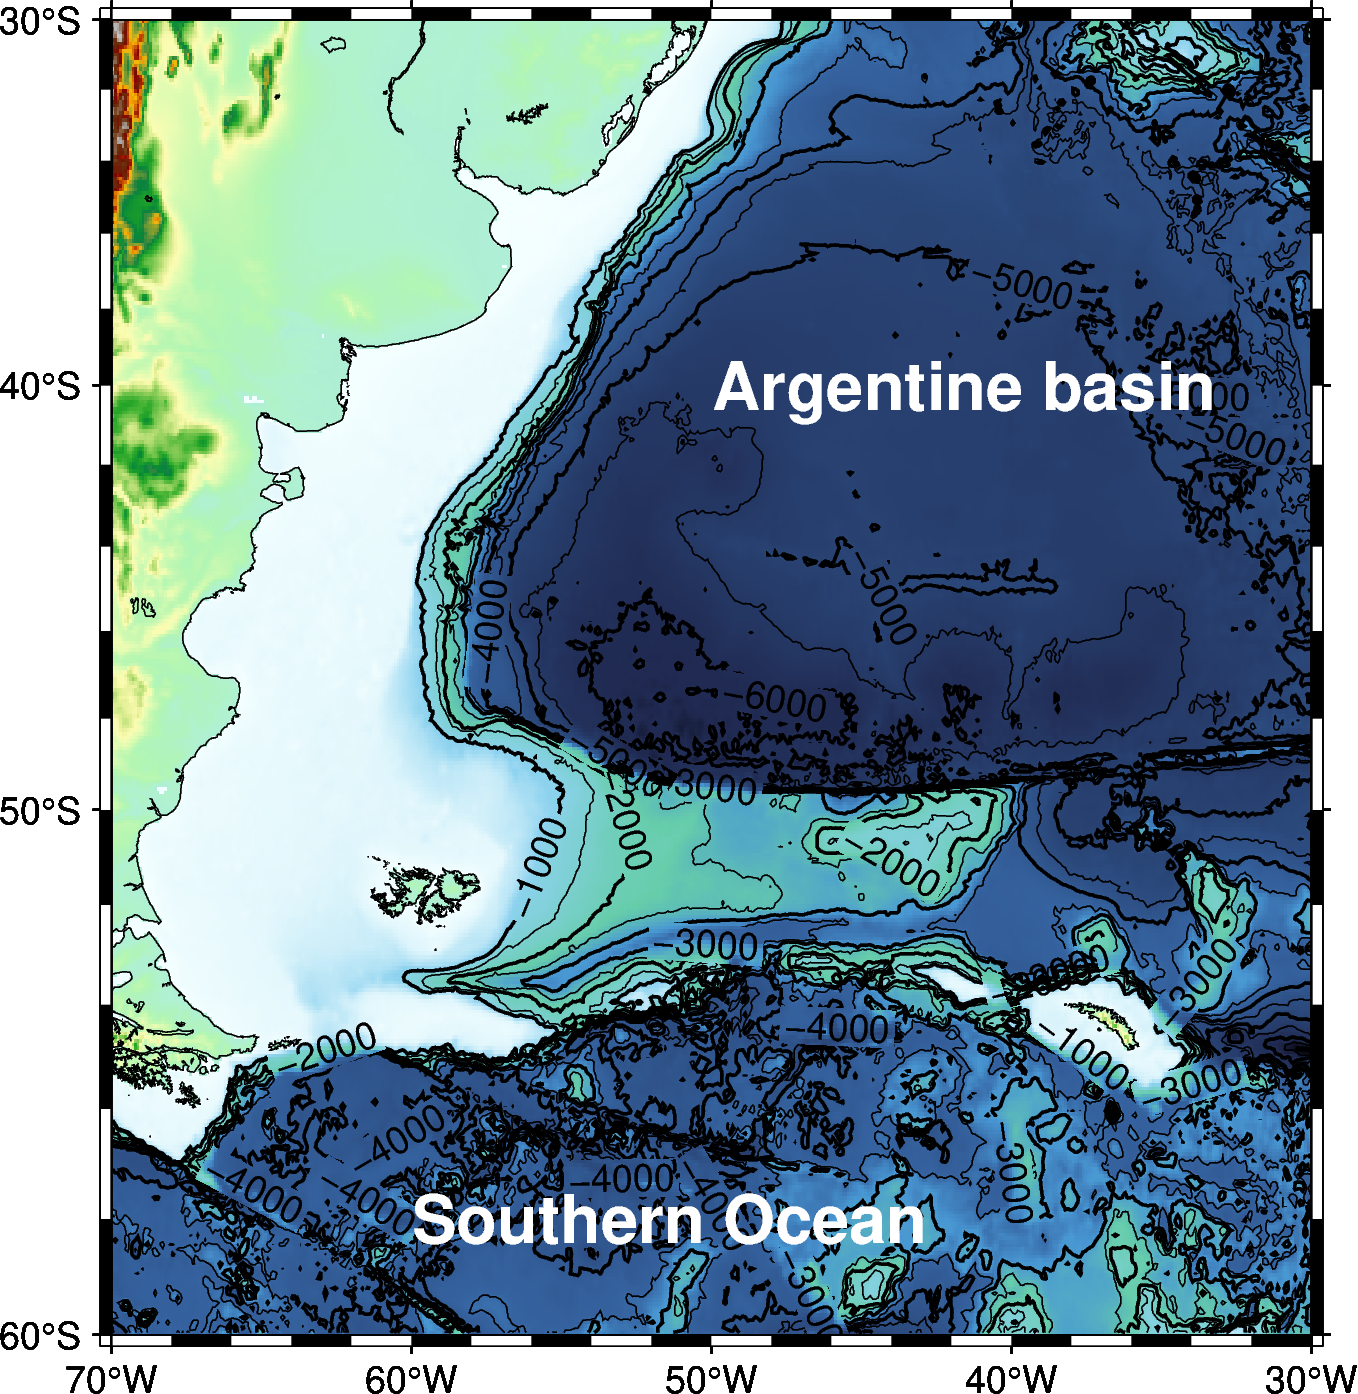
\includegraphics[width=15cm]{chapter/figure/research area topography map_earth.png}
  \caption
  {Topographic map of the research region}
  \label{research topography}
\end{figure}

The surface flow pattern of the research region is shown is figure \ref{surface flow pattern} and has already been descried in chapter \ref{flow pattern of the Argentine Basin} to show the importance of the study. Southward transport Brazil Current (BC) mix with northward transport Malvinas Current (MC) and form fluctuating Brazil/Malvinas Confluence (BMC) at about 40°S due to wind stress and baroclinic instabilities \cite{jullion2010circulation,weijer2015eddy}. An anticyclonic gyre called Zapiola Anticyclone (ZA) around the hill transports considerably large volume of water of about 200 Sv \cite{saunders1995bottom}. 

\begin{figure}[hbtp]
  \centering
  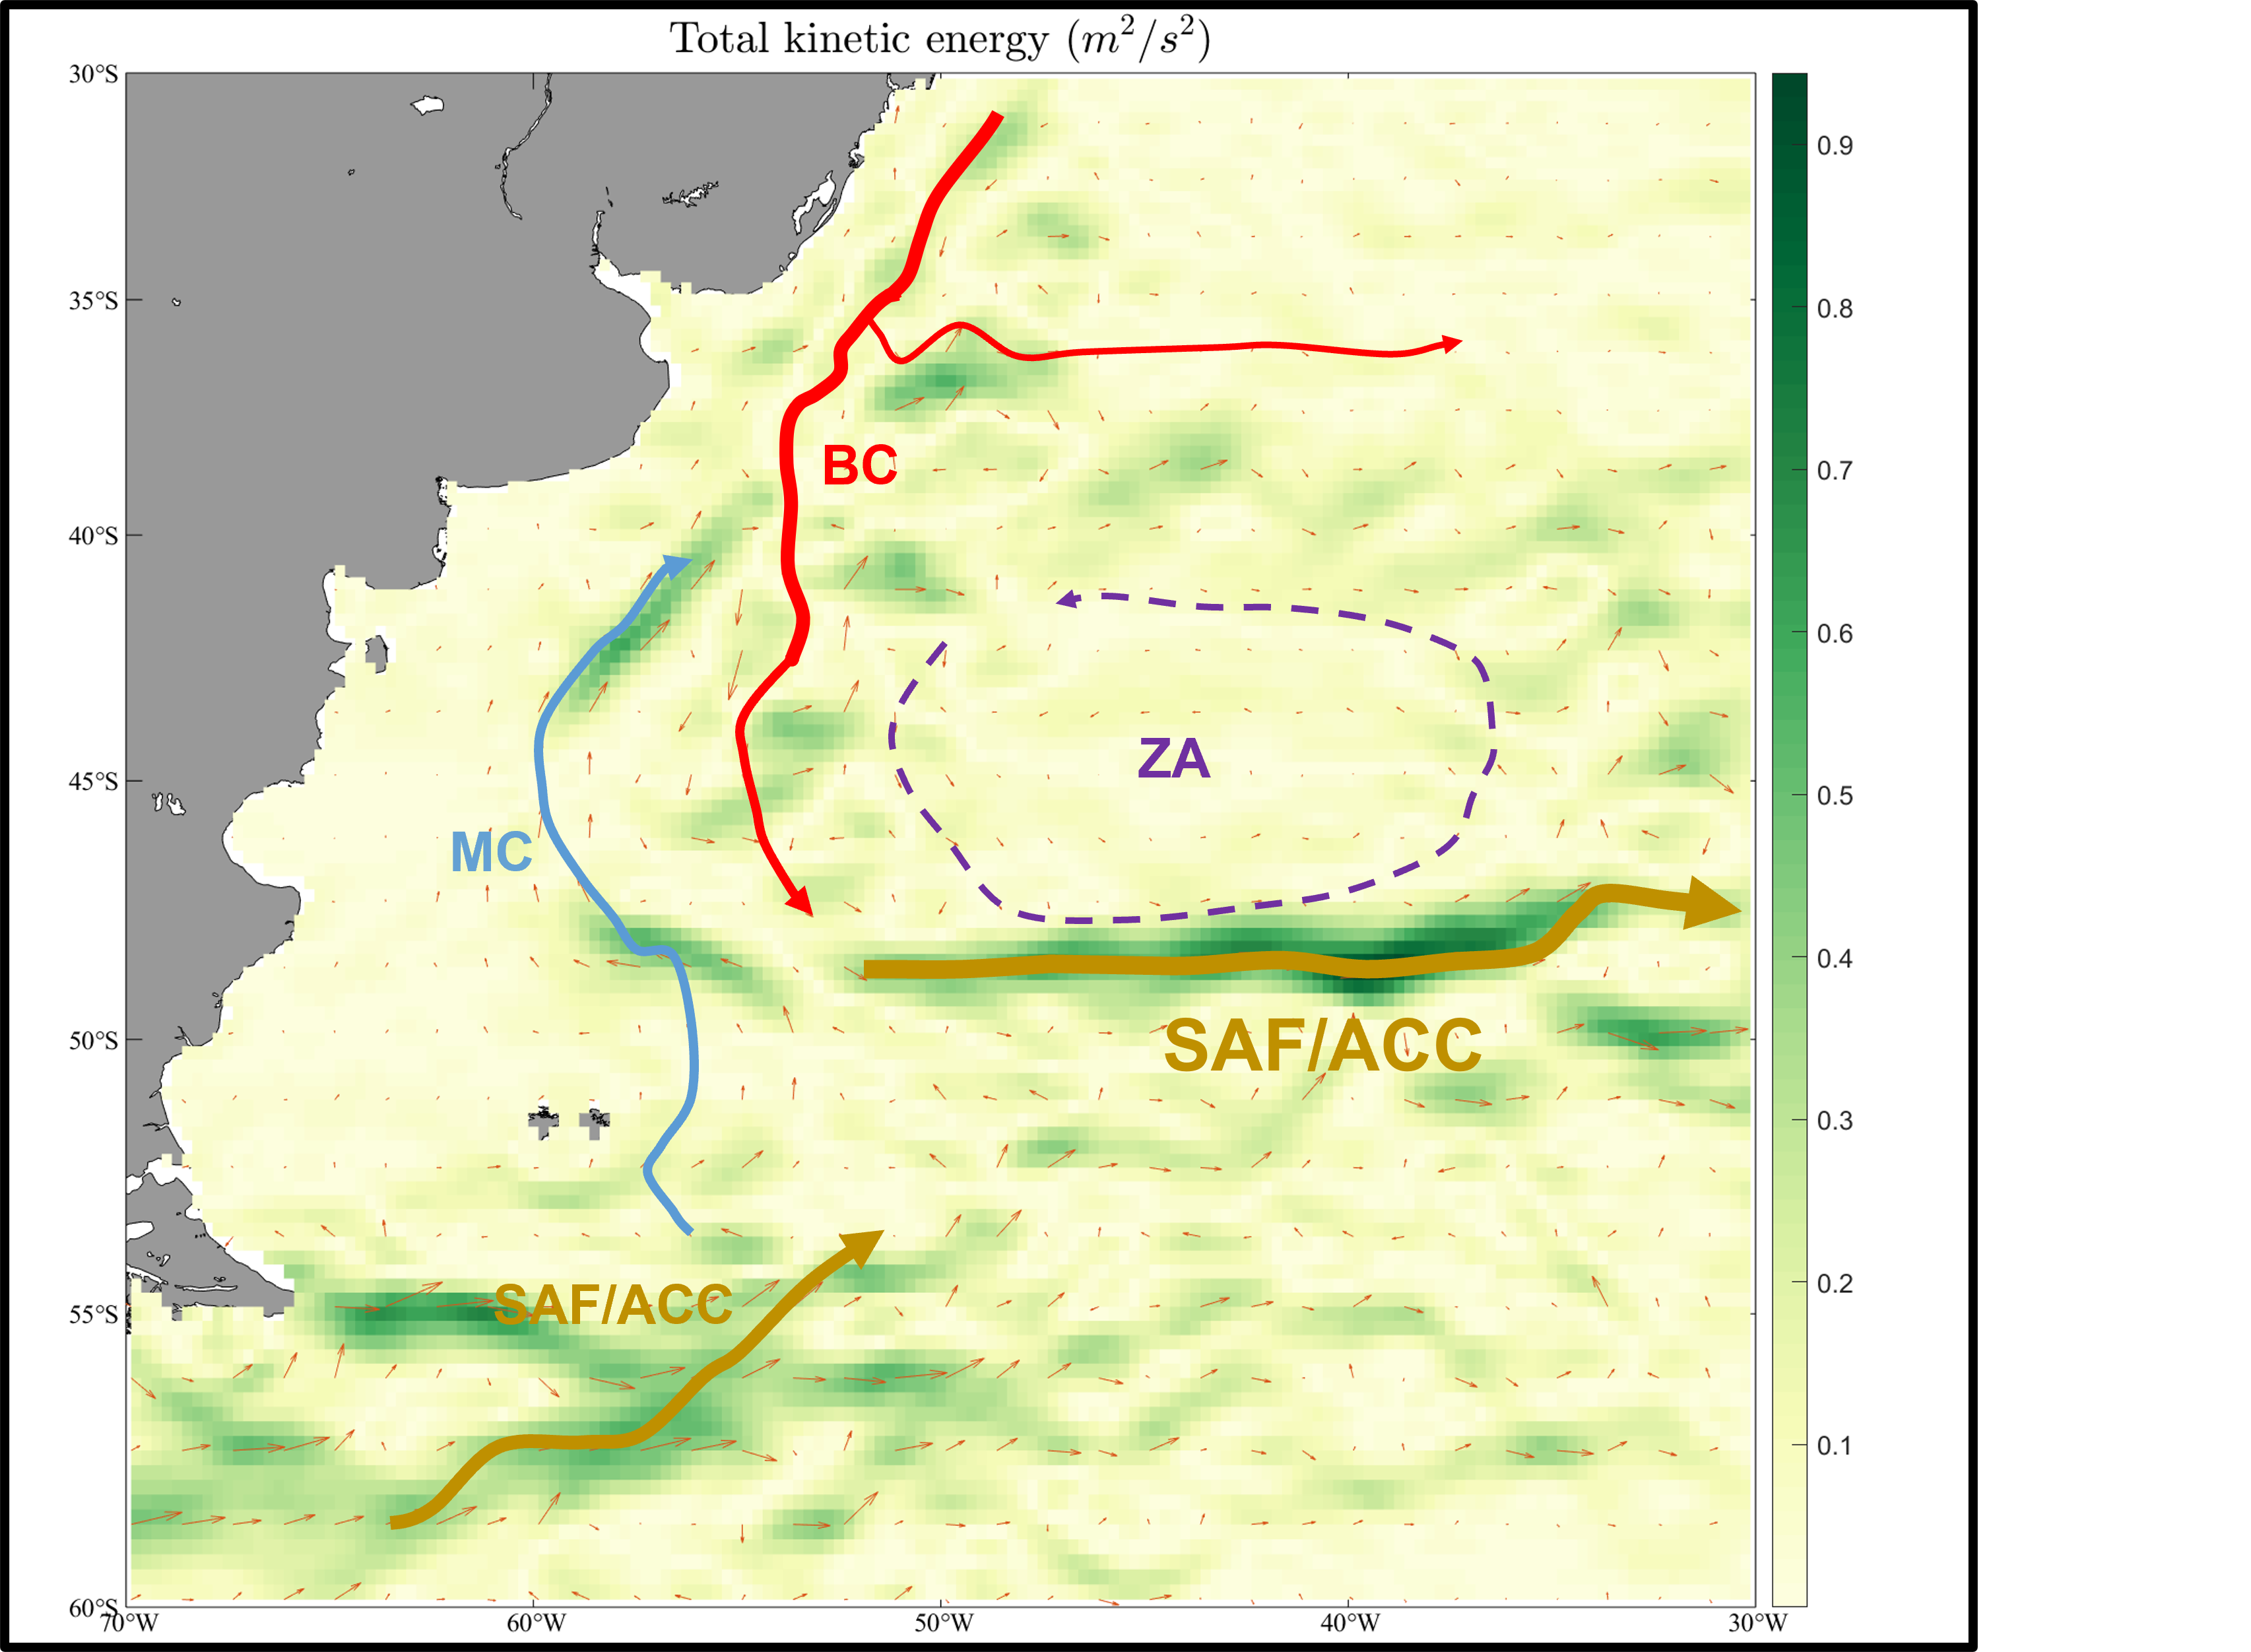
\includegraphics[width=15cm]{chapter/figure/surface flow with notion.png}
  \caption
  {Surface current pattern of the research area}
  \label{surface flow pattern}
\end{figure}

\section{Traditional Eulerian method and its drawback}

Since oceanic eddies are regarded as swirling bodies of water that trap a certain number of tracers inside, oceanic eddies are widely acknowledged to be Lagrangian (material).

There are two analytical frameworks for fluid mechanics study: one is the Eulerian method to describe the dynamics properties in a fixed space and the other is the Lagrangian method to describe the fluid properties from the point of view of particle motion \cite{kasten2011extraction}. 

Traditional eddy detection methods are Eulerian methods based on the instantaneous velocity field, which are not robust and may produce spurious results. For example, one of the Eulerian criteria is to seek a closed streamline in unsteady fluid flows; however, this topological feature is not invariant under Galilean transformations, and thus closed streamline may behave differently when choosing different Galilean transformation schemes \cite{kasten2011extraction}.

% Another way to extract vortex is based on scalar quantities such as $Q$ and $\lambda_2$, and these quantities are based on the Jacobian matrix of the flow field and thus are Galilean invariant.

As well as the above problems, Eulerian methods depend on the chosen thresholds value, thus the detection result could vary a lot when choosing different thresholds, generating noisy results and making the quantification of eddy transport unreasonable. 

\section{Objective Lagrangian eddies detection}\label{Lagrangian eddies detection}

In the last section, we discussed some Eulerian eddy-detection methods which are suitable for analysis of snapshot properties but not for distinguishing long-living structures from the incoherent unsteady flow.

Thus, more attention has been paid to the Lagrangian point of view and characterizes flow patterns in the path line.

The theory for extracting the material boundaries in steady or near-steady flow has been put forward for more than two decades; however, identifying material boundaries in unsteady flow has been a question for long time. Recently, Haller and Beron-Vera developed a new approach to describe transport barrier as the least stretching material line and the closed shearline of $\gamma_{t_0}$. The elliptic transport barrier is computed in the period of $[t_0,t+T]$, acting as the generalized KAM curve and conserving both its arclength and enclosed area until $t_0+T$ \cite{haller2012geodesic}. Thus, the elliptic transport barrier is the desired organization of the eddy candidate region.

The above theory seeks those frame-independent maximal shear as transport barriers and the shear barriers with a bunch of closed curves are called elliptic barriers \cite{wang2015identification}. The outermost elliptic barrier serves as the eddy boundary and enclosed the maximum area of coherent water mass over the domain\cite{wang2015identification}. 

\subsection{Computation setup}

We begin a two-dimensional velocity field $ \mathbf{v}(\mathbf{x},t)$, with $\mathbf{x}$ representing the position in the flow field and fix the time span ($[t_0,t_0+T]$) for tracking the coherent eddies.


\begin{equation}
    \dot{\mathbf{x}}(t)=\mathbf{u}(\mathbf{x}(t), t)
\end{equation}


For two-dimensional, divergence-free flows, we could introduce the stream function $\mathbf{\Psi}(x,y)$and rewrite the velocity in the form of gradient of the stream function. This conversion links the Hamiltonian mechanics and 2-D unsteady flow and makes the detection of invariant manifolds under the flow possible \cite{aref2017frontiers}.

\begin{equation}
    u=\frac{d x}{d t}=\frac{\partial \mathbf{\Psi}}{\partial y}, \quad v=\frac{d y}{d t}=-\frac{\partial \mathbf{\Psi}}{\partial x}
\end{equation}

We then introduce the concept of flow map $ F_{t_{0}}^{t_0+T} $. This map describes the Lagrangian trajectory of the particle released at initial position $x_0$ and how it evolves with time.

\begin{equation}
F_{t_{0}}^{t_0+T}: \mathbf{x}_{0} \mapsto \mathbf{x}\left(t_0+T;\mathbf{x}_{0}, t_{0}\right)
\end{equation}

In continuum fluid mechanics, we can describe the strain by introducing deformation gradient, and the following equation \ref{2-d DF} shows how to calculate deformation gradient in 2-dimensional flow fields.

%\begin{footnotesize} 
%\begin{align}
%    \nabla F_{t_{0}}^{t}\left(x_{0}\right) \approx\left(\begin{array}{cccc}
%\frac{x^{1}\left(t ; t_{0}, x_{0}+\delta_{1}\right)-x^{1}\left(t ; t_{0}, x_{0}-\delta_{1}\right)}{\left|2 \delta_{1}\right|} & \frac{x^{1}\left(t ; t_{0}, x_{0}+\delta_{2}\right)-x^{1}\left(t ; t_{0}, x_{0}-\delta_{2}\right)}{\left|2 \delta_{2}\right|} & \frac{x^{1}\left(t ; t_{0}, x_{0}+\delta_{3}\right)-x^{1}\left(t ; t_{0}, x_{0}-\delta_{3}\right)}{\left|2 \delta_{3}\right|} \\
%\frac{x^{2}\left(t ; t_{0}, x_{0}+\delta_{1}\right)-x^{2}\left(t ; t_{0}, x_{0}-\delta_{1}\right)}{\left|2 \delta_{1}\right|} & \frac{x^{2}\left(t ; t_{0}, x_{0}+\delta_{2}\right)-x^{2}\left(t ; t_{0}, x_{0}-\delta_{2}\right)}{\left|2 \delta_{2}\right|} & \frac{x^{2}\left(t ; t_{0}, x_{0}+\delta_{3}\right)-x^{2}\left(t ; t_{0}, x_{0}-\delta_{3}\right)}{\left|2 \delta_{3}\right|} \\
%\frac{x^{3}\left(t ; t_{0}, x_{0}+\delta_{1}\right)-x^{3}\left(t ; t_{0}, x_{0}-\delta_{1}\right)}{\left|2 \delta_{1}\right|} & \frac{x^{3}\left(t ; t_{0}, x_{0}+\delta_{2}\right)-x^{3}\left(t ; t_{0}, x_{0}-\delta_{2}\right)}{\left|2 \delta_{2}\right|} & \frac{x^{3}\left(t ; t_{0}, x_{0}+\delta_{3}\right)-x^{3}\left(t ; t_{0}, x_{0}-\delta_{3}\right)}{\left|2 \delta_{3}\right|}
%\end{array}\right)
%\label{3-d DF}
%\end{align}
%\end{footnotesize}

\begin{footnotesize} 
	\begin{align}
	\nabla F_{t_{0}}^{t}\left(x_{0}\right) \approx\left(\begin{array}{cccc}
	\frac{x^{1}\left(t ; t_{0}, x_{0}+\delta_{1}\right)-x^{1}\left(t ; t_{0}, x_{0}-\delta_{1}\right)}{\left|2 \delta_{1}\right|} & \frac{x^{1}\left(t ; t_{0}, x_{0}+\delta_{2}\right)-x^{1}\left(t ; t_{0}, x_{0}-\delta_{2}\right)}{\left|2 \delta_{2}\right|}  \\
	\frac{x^{2}\left(t ; t_{0}, x_{0}+\delta_{1}\right)-x^{2}\left(t ; t_{0}, x_{0}-\delta_{1}\right)}{\left|2 \delta_{1}\right|} & \frac{x^{2}\left(t ; t_{0}, x_{0}+\delta_{2}\right)-x^{2}\left(t ; t_{0}, x_{0}-\delta_{2}\right)}{\left|2 \delta_{2}\right|}  
	\end{array}\right)
	\label{2-d DF}
	\end{align}
\end{footnotesize}

In the above equation, $ \delta_{i} $ is a small vector pointing in the $ x^{i} $ coordinate direction.

The right Cauchy–Green strain tensor $\mathbf{C}_{t_{0}}^{t_{0}+T}\left(\mathbf{x}_{0}\right)$ is then
definded as 
\begin{equation}
    \mathbf{C}_{t_{0}}^{t_{0}+T}\left(\mathbf{x}_{0}\right)=\left(\nabla \mathbf{F}_{t_{0}}^{t_{0}+T}\left(\mathbf{x}_{0}\right)\right)^{\mathrm{T}} \nabla \mathbf{F}_{t_{0}}^{t_{0}+T}\left(\mathbf{x}_{0}\right)
\end{equation}


This symmetric tensor is positive definite, thus we could get two real positive eigenvalues $ \lambda_{i} $ and orthogonal real eigenvectors $ \xi_{i} $:

\begin{equation}
    C \xi_{i}=\lambda_{i} \xi_{i}, \quad\left|\xi_{i}\right|=1, \quad i=1, 2 ; \quad 0<\lambda_{1} \leq \lambda_{2}, \quad \xi_{i} \perp \xi_{j}, \quad i \neq j
\end{equation}

If the flow is incompressible, these two eigenvalues also satisfy the following relations:
 
\begin{equation}
     \operatorname{det} C=\prod_{i} \lambda_{i} \equiv 1,\quad0<\lambda_{1}<1<\lambda_{2}
\end{equation}



After setting up the invariant dynamical system, we now turn to scalar quantities.

The first technique is by using the Lyapunov exponent, which originates from dynamical system and measures how much close particles spread in the chaotic flow field. This method identifies LCSs as ridges in the Finite time Lyapunov exponent (FTLE) field and thus small or no material flux cross LCSs \cite{shadden2005definition, haller2001distinguished,haller2002lagrangian,haller2011lagrangian}. This method is widely used in ideal flow experiment.

The Finite time Lyapunov exponent $ \sigma $ is calculated as:

\begin{equation}
    \sigma\left(\mathbf{F}_{t_{0}}^{t_{0}+T}\left(\mathbf{x}_{0}\right) ; \mathbf{x}_{\mathbf{0}}\right)=\frac{1}{|T|} \log \sqrt{\lambda_{\max }\mathbf{C}\left(\mathbf{x}_{0}\right)}
\end{equation}

The second method is more rigorous mathematically and identifies the least stretching or deforming material surface (in 3-D flow) or material line (2-d flow) through a variational theory\cite{blazevski2014hyperbolic,haller2011variational,haller2012geodesic}. This method is more widely used in geophysical flows and recent studies of life cycle of a coherent Agulhas ring and detection of Agulhas Leakage have demonstrated its robustness\cite{wang2015identification,wang2016life,beron2013objective}. 
First, we assume an initial materine line to be $\mathcal{M}(t_0)$ and then it is advected to be $\mathcal{M}(t_0+T)$ according to equation \ref{material line}.

\begin{equation}
    \mathcal{M}(t_0+T):=F_{t_{0}}^{t_0+T}\left(\mathcal{M}\left(t_{0}\right)\right)
    \label{material line}
\end{equation}

To express this coherence principle mathematically, we select a parametrization $r(s)$ with $s \in[0, \sigma]$ for the closed curve $\gamma$ at time $t_{0}$, and denote the length of a tangent vector $r^{\prime}(s)$ by $l_{t_{0}}(s)$. We also let $l_{t_0+T}(s)$ denote the length of the corresponding tangent vector $(\mathrm{d} / \mathrm{d} s) F_{t_{0}}^{t_0+T}(r(s))$ along the advected curve $F_{t_{0}}^{t_0+ T}(\gamma) .$ These two tangent lengths can be calculated as

\begin{equation}
    l_{t_{0}}(s)=\sqrt{\left\langle r^{\prime}(s), r^{\prime}(s)\right\rangle}, \quad l_{t}(s)=\sqrt{\left\langle r^{\prime}(s), C_{t_{0}}^{t}(r(s)) r^{\prime}(s)\right\rangle}
\end{equation}

\begin{figure}[ht]
  \centering
  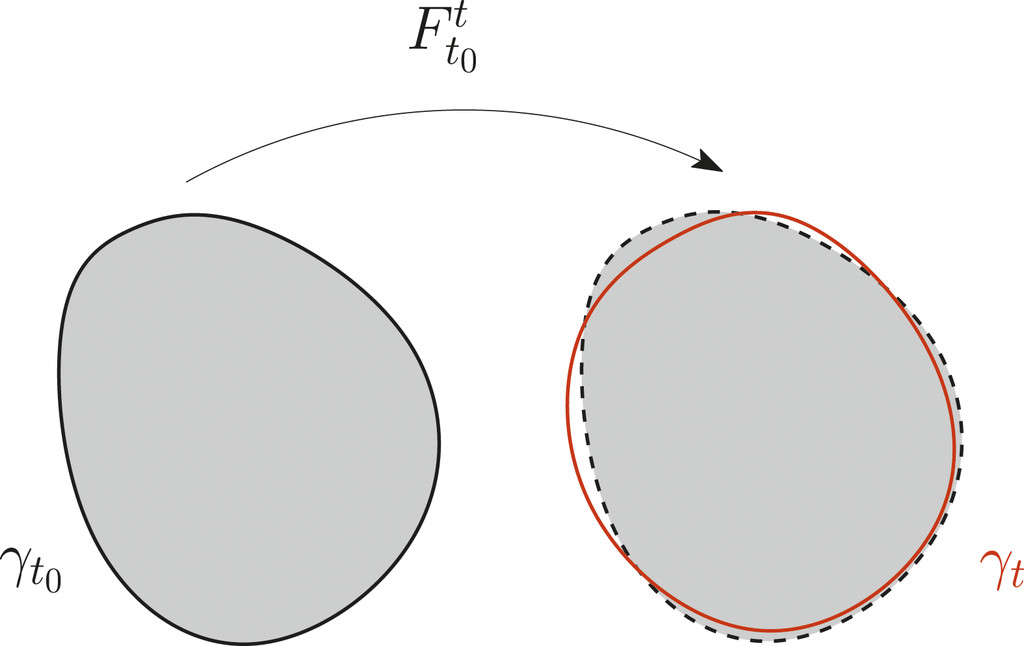
\includegraphics[width=15cm]{chapter/figure/Schematics of a closed shearline.jpg}
  \caption
  {Schematic of a closed shearline (elliptic transport barrier) \cite{beron2013objective}
  }
\end{figure}

where $\langle\cdot, \cdot\rangle$ denotes the Euclidean inner product \cite{truesdell2004non}. The averaged tangential strain along $\gamma$ is then given by

\begin{equation}
    Q(\gamma)=\frac{1}{\sigma} \int_{0}^{\sigma} \frac{l_{t_0+T}(s)}{l_{t_{0}}(s)} \mathrm{d} s
\end{equation}


As argued above, if an observable coherent material belt exists around $\gamma$, then on $\varepsilon$-close material loops we must have $Q(\gamma+\varepsilon h)=Q(\gamma)+O\left(\varepsilon^{2}\right)$, where $\varepsilon h(s)$ denotes small, periodic perturbations to $\gamma$. This is only possible if the first variation of $Q$ vanishes on $\gamma$ :

\begin{equation}
  \delta Q(\gamma)=0
\end{equation}


\begin{figure}[ht]
  \centering
  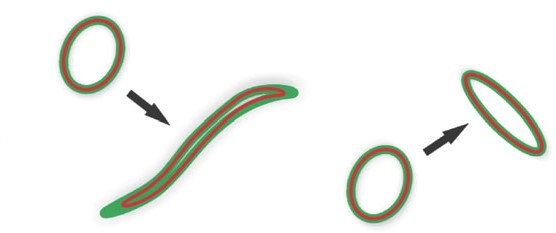
\includegraphics[width=15cm]{chapter/figure/Haller_Beron-Vera_2013_Coherent Lagrangian vortices_Journal of Fluid Mechanics.jpg}
  \caption
  {Comparison of ordinary material line and coherent material line \cite{haller2013coherent}
  }
  \label{material line compare}
\end{figure}

The third method for detecting the oceanic eddies is the Lagrangian Averaged Vorticity Deviation (LAVD) method, which is more intuitive and takes the time-integrated deviation of vorticity from background vorticity into consideration \cite{haller2016defining,tarshish2018identifying}. Using this method, vortex center is regarded as the maximum value of $|LAVD|$ and the vortex boundaries are the outermost convex curves around the center. We define coherence over a finite time interval $[t_0,t_0+T]$, which means that water column remain inside vortex during the period.


\begin{equation}
    LAVD_{t_0}^{t_0+T}(x_{0})=\int_{t_0}^{t_0+T}|\omega-\bar{\omega}| d s \quad 
\end{equation}

In the study, we apply LAVD eddy detection algorithm to altimetry-derived ocean currents starting on the first day of every month from 1993-2019, and the coherence time spans is 30 days. In the next step, we also change the time period from 30 days to 60 days, 90 days, and even 120 days and apply the methods to the model simulation product at each depth. Tracking coherent eddies in a 27-year period contributes to the understanding of the role of oceanic eddies in the transport process, especially the move of diffusive material and climatology trend of eddies change. The coherence time span varies to test the maximum material coherence of the eddies.

%We adopt fourth-order Runge–Kutta method in the interpolation process to get the eddy trajectories.

Thus, the workflow for us to apply the eddy detection algorithm to extract oceanic eddies from the flow field is as follows:

\begin{itemize}
  \item [1)] 
  Set up a two-dimensional velocity field to advect the particle.
  \item [2)]
  Introduce the definition of flow map to show how particles move in the coherent time interval $\Delta t$.
  \item [3)]
  Calculate the deformation gradient and get the Cauchy-Green Strain Tensor.
  \item[4)]
  Finally, we compute the LCSs from the LAVD field.
\end{itemize}

%Besides, we also use Eulerian methods in the study to validate the robustness of the result.

% \subsection{Calculation of eddies transport}

% \section{Some statistics about vortex}

% After setting up the dynamical system, and detecting the vortex center and boundary from the flow, we could compute some properties of the vortex.
% The area A of the vortex refers to the boundary contained within the boundary of the vortex, and the radius R is regarded as the radius of a circle of the equal area $R = \sqrt{A/\pi}$.

% Geostrophic velocity anomaly was shown in equation \ref{Geostrophic anomaly velocity}, which is derived from the gradient of the SLA. Eddy kinetic energy (EKE) is half of the sum of the squares of the geostrophic velocity anomaly:

% \begin{equation}
%     EKE=\frac{1}{2}\left(u^{\prime 2}+v^{\prime 2}\right)
% \end{equation}

% After calculating the EKE, we could then define a parameter called eddy intensity to describe the average eddy kinetic energy normalized by vortex area.

% \begin{equation}
%     EI=\frac{\langle EKE\rangle}{A}=\frac{\langle EKE\rangle}{\pi R^{2}}
% \end{equation}





\newpage
